%!TEX root = main.tex
% 159 words
\chapter{Plan of Remaining Work} % (fold)
\label{cha:plan_of_remaining_work}

% Emphasize the modularity of the project, split stuff up

% contingency plans - what may go wrong? So much... FPGA too big, ARM board doesn't work, System too complex / hard to port to FPGA, not enough memory on FPGA

\section{Overview} % (fold)
\label{sec:overview}
Since the start of the project there has been a number of decision changes, as the scope and challenges of the project became more clear.  The initial plan (Figure~\ref{fig:gantt1}) was unrealistic in some senses, and a revised Gantt chart \footnote{Both Gantt charts were created and modified using Gantter (http://app.gantter.com)} has been created for the remaining work (Figure~\ref{fig:gantt2}). 

A notable difference between the first and second Gantt charts is that the first made far fewer attempts to break the implementation work up.  In addition, it underestimated the time that would be required to set up the L'Imperatrice board.  Finally, more time has been allowed to do the project report, as more time should have been given to writing the interim report.

The second plan is designed to split the remaining work in such a way that there is less dependence between tasks.  If at all possible the work is modularised, so that if one section becomes unfeasible, it can be dropped without affecting the outcome of the final product greatly.


\begin{figure}[tb]
	\begin{center}
		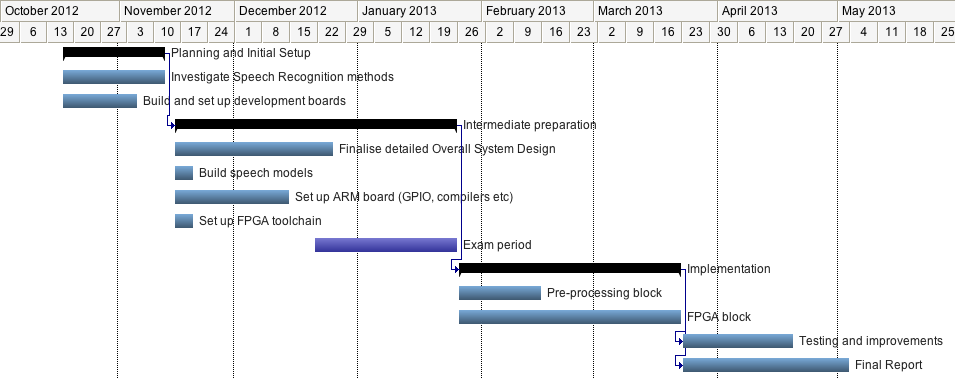
\includegraphics[width=1.4\textwidth,angle=90]{gantt-chart-initial.png}
	\end{center}
	\caption{First Gantt chart with high expectations}
	\label{fig:gantt1}
\end{figure}

\begin{figure}[tb]
	\begin{center}
		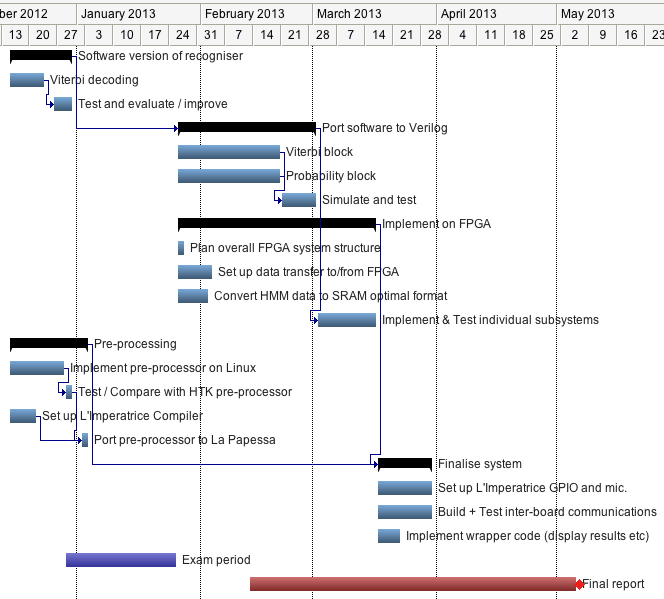
\includegraphics[width=1.1\textwidth,angle=90]{gantt-chart-interim.png}
	\end{center}
	\caption{Interim Gantt chart for remaining work}
	\label{fig:gantt2}
\end{figure}
% section overview (end)


\section{Considerations} % (fold)
\label{sec:details_of_tasks}
In the event that pre-processing code is too hard or time consuming to write, the alternative is to use the HTK to do it, and test the speech recognition offline.  Initialy all development of the system will use the HTK generated MFCC files, as there is certainty that they are correct.  This will allow focus to remain on the more interesting problem of implementing a viterbi decoder block in hardware.

The Voxforge models may be far too complex to use for the project, as straightforward Viterbi decoding is not sufficient for larger models.  If this is the case, there are several options that have been investigated, and neither would take much time.  The HTK is capable of reducing model size by using clustering and regression trees.  Another option would be to train a very simple model from scratch, possibly using the audio and transcriptions available on Voxforge.  However, the priority is to build the system, and if the model is found to be too large it can be adapted.

It may be that the Spartan 3AN FPGA on La Papessa will be too small to hold the system code.  If this is the case, the University has several Altera DE0 evaluation boards that have much more space, with the only downside being that this moves away from the Micro Arcana family.  

% section details_of_tasks (end)


% chapter plan_of_remaining_work (end)